% This is samplepaper.tex, a sample chapter demonstrating the
% LLNCS macro package for Springer Computer Science proceedings;
% Version 2.20 of 2017/10/04
%
\documentclass[runningheads]{llncs}
%
\usepackage{graphicx}
\usepackage[spanish]{babel}
\usepackage[utf8]{inputenc}
\usepackage[hidelinks,breaklinks=true,backref=page]{hyperref}
% Used for displaying a sample figure. If possible, figure files should
% be included in EPS format.
%
% If you use the hyperref package, please uncomment the following line
% to display URLs in blue roman font according to Springer's eBook style:
% \renewcommand\UrlFont{\color{blue}\rmfamily}

\begin{document}
%
\title{Motor de Búsqueda: Modelo Vectorial y Ranking SVM}
%
%\titlerunning{Abbreviated paper title}
% If the paper title is too long for the running head, you can set
% an abbreviated paper title here
%
\author{Luis Ernesto Ibarra Vázquez\inst{1} \and
Luis Enrique Dalmau Coopat\inst{2} \and
Adrian Hernández Pérez\inst{3}}
%
\authorrunning{Luis Ibarra, Luis Dalmau, Adrian Hernández}
% First names are abbreviated in the running head.
% If there are more than two authors, 'et al.' is used.
%
\institute{Universidad de La Habana, La Habana, Cuba\\
\url{https://www.uh.cu}}
%
\maketitle              % typeset the header of the contribution
%
\begin{abstract}
% The abstract should briefly summarize the contents of the paper in
% 150--250 words.
La creación de motores de búsqueda permiten a los usuarios acceder a la información
que buscan de manera rápida y eficiente. Este trabajo presenta una implementación de 
un motor de búsqueda basado en el modelo vectorial y en Ranking SVM. Se presentan la arquitectura,
algoritmos y procesamientos usados para dicha implementación. Se trabajó sobre un conjunto de datos
de tipo científico obteniendo resultados superiores en el modelo vectorial y se evidencia el efecto
del algoritmo de Rocchio para el mejoramiento de las métricas en la retroalimentación del motor de búsqueda.
El resultado final es presentado al usuario mediante una interfaz gráfica que permite
al usuario realizar consultas de manera natural.

\keywords{Recuperación de Información  \and Motor de Búsqueda \and Modelo Vectorial. \and Support Vector Machine}
\end{abstract}

\section{Introducción}

El ámbito de recuperación de información es un área de las Ciencias de la Computación que tiene
actualmente gran importancia debido al gran volumen de información que se genera cada día en la
web. Esta información debe de ser encontrada por los usuarios de manera rápida y eficiente y es
de esta tarea en la cual un motor de búsqueda es necesario. La tarea esencial de un motor de
búsqueda es la de recuperar documentos que estén asociados a una pregunta planteada por el usuario, 
esta recuperación tiene que ser de calidad conteniendo información relevante que el usuario pueda
usar para lograr su objetivo.

En este ámbito se presentan tres tipos de modelos clásicos de recuperación de los
cuales surgen nuevas variantes, los tipos son:

\begin{itemize}
    \item Vectorial
    \item Probabilístico
    \item Booleano
\end{itemize}

El objetivo del trabajo consiste en la implementación y evaluación de un motor de búsqueda,
en este caso se usa el modelo vectorial y el modelo de Ranking SVM. Además es necesario la
construcción de una interfaz visual para la interacción con el usuario, en este caso se usó
streamlit y Flutter para la construcción de páginas web con esta finalidad.

El trabajo de divide en varias secciones, primero se analiza la arquitectura del motor de
búsqueda, se presenta el algoritmo y procesamiento usado para la implementación de 
este, presentará una sección sobre la implementación de la interfaz gráfica, por último
se presenta el resultado final del motor de búsqueda.

\section{Arquitectura}

Todo motor de búsqueda consta de tres partes fundamentales a la hora de darle respuesta al usuario

\begin{itemize}
    \item Recibir una pregunta
    \item Buscar documentos relevantes a la pregunta
    \item Devolver los documentos relevantes encontrados
\end{itemize}

\subsection{Flujo de datos del motor de búsqueda}

El motor de búsqueda es el núcleo fundamental de la implementación. Un problema fundamental que
tiene la etapa de desarrollo es que en esta se realizan muchos cambios en el código fuente agregando
o cambiando funcionalidades al procesamiento, además estas funcionalidades generalmente se pueden usar
de manera independiente para otros procesamientos como por ejemplo la implementación de otro modelo
dentro del mismo motor de búsqueda. Para poder resolver este problema de una manera sencilla se estructura
el proyecto mediante una arquitectura de tuberías o flujos (pipelines). Esta arquitectura consiste en una serie
de tuberías que se conectan entre sí, pasando un contexto entre ellas y combinando de forma desacoplada
los resultados obtenidos de cada tubería. Un ejemplo de lo anterior es que la lectura de los documentos
es independiente de su procesamiento así que si se quiere cambiar esta funcionalidad es solamente necesario
cambiar el pedazo del flujo encargado de esto, otro ejemplo de las ventajas es que el proceso de
tokenización de los documentos generalmente es el mismo, en el caso de que se quieran implementar varios
modelos se puede reutilizar este flujo sin mucho esfuerzo y manteniendo la misma arquitectura (Figura \ref{pipeline_fig}).


\subsection{Comunicación con el motor de búsqueda}

La comunicación del motor de búsqueda con el exterior se hace a través de una API REST. Con esta
es posible preguntarle al motor de búsqueda y que este devuelva las respuestas asociadas. Gracias
a que la comunicación se hace mediante HTTP es posible realizar la implementación de varios clientes
que consuman de esta y que presenten la información de la manera que más le convenga al cliente.\\

Los principales endpoints de esta interfaz son:

\begin{itemize}
    \item GET \url{search/?query=query\&offset=offset} Devuelve una lista asociada a los
documentos relevantes de la búsqueda.
    \item GET \url{document/?document\_dir=document\_dir} Devuelve el contenido del documento asociado
al id dado.
	\item GET \url{expand/?query=query} Devuelve las posibles expansiones de consulta encontradas por el programa
	\item POST \url{feedback/} Envía la información para marcar como relevante o no los documentos mostrados.
\end{itemize}

\section{Implementación del motor de búsqueda}

\subsection{Tokenización}

La tokenización es el proceso en el cual se divide una cadena de caracteres en palabras o tokens.
Estos tokens son luego procesados en dependencia del modelo de búsqueda que se quiera implementar.
La implementación de la tokenización en el motor de búsqueda se lleva a cabo mediante el uso del
framework nltk. Esta es dividida principalmente en varias etapas:

\begin{enumerate}
    \item Convertir el texto en tokens
    \item Limpiar los tokens
    \item Remover las stopwords
    \item Aplicar raíz semántica a los tokens con Wordnet
    \item Aplicar stemming o lemmatizing a los tokens
\end{enumerate}

Mediante estos proceso se llega al final de esta etapa con una lista de tokens procesada la cual
representa el documento. Esta lista es luego convertida a la representación necesitada en cada modelo
para su procesamiento.

Este procesamiento puede ser el mismo independientemente del tipo de modelo utilizado.

\subsection{Modelo Vectorial}

El modelo vectorial se centra en la idea de que la relevancia de los documentos con la consulta está 
dada por las palabras que contienen. Para esto se encuentran representaciones vectoriales de ambos
para que se pueda hacer la comparación. En el modelo planteado en el trabajo se hace una implementación
del modelo clásico vectorial el cual no toma en cuenta el orden de las palabras en su representación, haciendo
de este un modelo estilo bolsa de palabras.

\subsubsection{Representación de los documentos}

Para el procesamiento del modelo vectorial se utiliza una representación de documentos en forma de
vectores. Esta representación se obtiene a partir de la tokenización previa de los documentos. La
representación de los documentos se obtiene a partir de la siguiente fórmula:

\begin{equation}
    w_{ij} = \frac{tf_{ij}}{\max_{k} tf_{kj}}idf_{j}
\end{equation}

Donde $w_{ij}$ representa el peso asociado al término $i$ en el documento $j$ y $tf_{ij}$ el número de veces que
se repite el término $i$ en el documento $j$. $idf_{j}$ es la frecuencia inversa del documento $j$ en la
colección de documentos calculada por $\log{\frac{N}{n_j}}$ donde $n_j$ es la cantidad de documentos
en donde aparece el término $j$.

\subsubsection{Representación de la consulta}

La representación de la consulta en el modelo vectorial es la misma que la representación de los 
documentos, pero con una diferencia que se aplica una fórmula diferente.

\begin{equation}
    (\alpha idf_i + (1-\alpha)\frac{tf_{ij}}{\max_{k} tf_{kj}}) idf_i
\end{equation}

En este caso $\alpha$ es un hiperparámetro para suavizar cuyo rol es disminuir
la contribución del segundo término \cite{alphaManning}. En la práctica dicho parámetro
se especificó a 0 luego de probar varios valores.

\subsubsection{Ranking de documentos}

Para el ordenamiento de los documentos se utiliza la representación de la consulta y de los documentos
en su forma vectorial. Para el cálculo de la similitud entre ambas se utiliza el coseno entre
ambos vectores:

\begin{equation}
    sim(q,d_i) = \cos(q, d_i) = \frac{q \cdot d_i}{||q|| ||d_i||}
\end{equation}

Una vez se tienen estos valores se ordenan de mayor a menor y son devueltos en ese orden al
usuario.

\subsection{Modelo Ranking SVM}

El modelo Ranking SVM se basa en que los documentos y las consultas se pueden representar como vectores
en los cuales se guarda información acerca de sus características e interacciones. Inicialmente
el problema resuelto por SVM es uno de clasificación, por lo que se tendría que convertir
el problema de Ranking a uno de clasificación. Para esto se considera la siguiente idea, se
entrenará el modelo SVM para detectar si un documento es más relevante a otro con la misma query.
Para la implementación de dicho algoritmo se usó los SVM de sklearn.

\subsubsection{Representación de Documentos y Consultas}

Dado que el modelo necesita tener información acerca de la consulta y su relación con el documento,
se modela una representación conjunta de ambos. Esta representación conjunta puede guardar todo tipo
de información aunque en el trabajo se representa por la concatenación de los siguientes aspectos:

\begin{itemize}
	\item Coseno entre la representación vectorial TF-IDF de la consulta y el documento
	\item Distancia euclidiana entre la representación vectorial TF-IDF de la consulta y el documento
	\item Cantidad de palabras que aparecen en la consulta y el documento
	\item Similitud de Jacard entre los tokens de la consulta y del documento
	\item Coseno entre el vector TF-IDF reducido de la consulta y del documento mediente descomposición SVD
	\item Distancia euclidiana entre el vector TF-IDF reducido de la consulta y del documento mediente descomposición SVD
\end{itemize}

La descomposición de SVD se basa en el proceso de Latent Semantic Analysis (LSA) cuyo objetivo 
consiste en reducir la dimensionalidad de los términos aplicándole la descomposición SVD a la
matriz de TF-IDF generada en orden de obtener una representación más compacta y que guarde 
información semántica de los términos \cite{lsaWiki}.

Se intentó usar directamente el vector LSA de la consulta y del documento como feature en el entrenamiento,
el resultado fue que los pesos asociados a la consulta quedaban nulos, por lo tanto esta no influía en el
resultado así que esta idea quedó descartada.

\subsubsection{Ranking de los documentos}

Para la conversión del problema de ranking a uno de clasificación se parte de la siguiente
hipótesis en el espacio del trabajo con SVMs:


\begin{equation}
w\theta_{iq} > w\theta_{jq} \iff r_q(d_i) > r_q(d_j)
\end{equation}

Donde:

\begin{itemize}

	\item $w$: Son los pesos encontrados de aplicar SVM al conjunto de entrenamiento
	\item $\theta_{iq}$: Es la representación conjunta del documento i con la query
	\item $r_q(d_i)$: Es la relevancia del documento i con respecto a la query
	
\end{itemize}

Partiendo de lo anterior se tiene que:

\begin{equation}
w(\theta_{iq} - \theta_{jq}) > 0 \iff r_q(d_i) - r_q(d_j) > 0
\end{equation}

Lo que en términos de SVM equivale a encontrar el hiperplano que maximiza la distancia entre las distintas clases
del vector diferencia visto anteriormente.

Con lo anterior se tiene un clasificador que contiene información de qué hace que los documentos y las 
consultas sean relevantes o no, encontrando un separador que maximiza el margen entre estas diferencias.

Para el orden de los documentos dado una consulta se propone el siguiente criterio, en donde los documentos son
ordenados de mayor a menor por el valor del resultado \cite{rankSVM}:

\begin{equation}
rsv(q, d_i) = w^* \theta_{iq}
\end{equation}

\subsubsection{Elección del kernel SVM}

En la elección del tipo de SVM a utilizar se probaron diferentes kernels, el linear, polinomial y RBF, con estos
se obtuvieron resultados similares, dado que el linear es más simple y rápido y los otros no aportaban un aumento
significativo se decidió dejar este \cite{svmSklearn}.

\subsubsection{Entrenamiento}

Para el entrenamiento final obtuvo una precisión del 57\% por lo que nos indica que la separación no es buena con
los atributos propuestos. Puede ser que al encontrar un conjunto de atributos que separe correctamente los documentos
se logre mejorar el rendimiento del modelo.

\subsection{Retroalimentación}

Para la retroalimentación se eligió el algoritmo de Rocchio debido a su simplicidad. Este se basa 
en el cálculo de centroides de un conjunto de documentos relevantes y no relevantes a una query
y su posterior suma ponderada con el objetivo de mover el vector query hacia el conjunto de 
documentos relevantes y alejarlo del conjunto de documentos no relevantes. La fórmula final sería:

\begin{equation}
    q_f = \alpha q_0 + \frac{\beta}{|D_r|}*\sum_{d_r \in D_r} d_r -  \frac{\gamma}{|D_{nr}|}*\sum_{d_{nr} \in D_{nr}} d_{nr} 
\end{equation}

Dado que la relevancia depende de la query, se crea una estructura de datos la cual guarda esta correspondencia. 
En un principio esta estructura de datos solamente guarda los vectores relevantes o no que coincidan exactamente
con la query, aunque se ideó una variante de esta estructura para devuelver los documentos relevantes y no
relevantes, para ser usado en el algoritmo de Rocchio, que estén en una zona cercana no exacta, aumentando así el recuperado de estos documentos.

Se utilizan para dicho algoritmo toda la información acerca de los documentos relevantes y los no 
relevantes para una determinada consulta(y la de consultas similares a esta en nuestro caso) para 
acercar más a dicha consulta a la zona de los documentos relevantes y alejarla de los documentos no 
relevantes. Se utilizan los valores usuales de alpha,
beta y ro los cuales son 1, 0.75 y 0.1 respectivamente. 

La retroalimentación también está dada explícita por el usuario. Se puede crear el modelo realizando 
un sembrado automático de las relaciones consulta-documento del corpus las cuales sirven para, dada la 
consulta, encontrar consultas similares a estas y devolver los documentos relevantes y no relevantes 
para utilizar en el algoritmo de Rocchio. Se utiliza un valor preestablecido de 0.25 para separar las 
consultas similares más significativas y además solo se escogen las 5 primeras consultas con mayor 
similitud, incluyendo a la misma consulta para poder tomar en cuenta la retroalimentación dada por el 
usuario.


%TODO Implementar esta última idea, ver qué funciona mejor y ponerlo en el informe

\subsection{Expansión de query}

Para implementar la expansión de query se hizo un algoritmo de correlación de términos, donde se analiza la última palabra de la 
query, y si está en algún documento, entonces se hace un ranking de las palabras que más se usan después de esa palabra en los
documentos. Para hacer esto se hizo una matriz para la correlación de los términos, de dimensión NxN donde N es la cantidad de 
palabras diferentes en el corpus, donde el valor en $[x,y]$ representa la cantidad de veces que después de la palabra $x$ está 
la palabra $y$, se utilizó una matriz esparcida, que es una estructura muy útil para esto, ya que los valores que son 0 en la 
matriz, o sea los valores que no se han modificado no se guardan en memoria, y esta matriz cumple la característica de que la 
mayoría de sus valores son cero, y esto representa eficiencia y un gran ahorro de memoria. Con la matriz de correlación se saca 
el ranking de palabras ordenando la fila asociada a $x$ por sus valores de mayor a menor y devolviendo los términos asociados a 
los primeros elementos del ordenamiento.

\section{Interfaz gráfica}

\subsection{Flutter}

La interfaz gráfica actúa como un cliente REST que consume los servicios de búsqueda. Esta
se presenta como un navegador web que le permite realizar todas las interacciones necesarias
con el motor de búsqueda Figura \ref{ui_fig}.

Entre las acciones posibles a realizar se encuentran:

\begin{itemize}

\item Hacer una consulta.
\item Ver el contenido de un documento.
\item Dar feedback mediante like o dislike.

\end{itemize}

\subsection{Streamlit}

La interfaz gráfica de streamlit consume directamente del código escrito, por lo que se 
integra más fácil con los nuevos cambios que la versión de Flutter Figura \ref{ui_streamlit_fig}.

Entre las acciones posibles a realizar se encuentran las mismas que las de Flutter aunque se le
agregan otras:

\begin{itemize}

\item Ver las expansiones de consulta.
\item Ver las consultas asociadas al corpus con que se está trabajando
\item Ver la relevancia de la consulta (si es textual del corpus) sobre los 
documentos devueltos en el corpus con que

\end{itemize}

\section{Evaluación}

Para la evaluación del motor de búsqueda se utilizaron dos corpus. El primero de estos
es el corpus de Cranfield, este contiene los resúmenes de 1400 artículos científicos, además
de tener unas 225 consultas con 1800 relaciones de relevancia entre estas y los documentos anotados.
El otro corpus usado es el Med, el cual contiene 1033 archivos que tratan sobre resúmenes de investigaciones
médicas, este presenta 30 consultas las cuales se relacionan 696 veces con los documentos, siendo estas
relaciones todas positivas.

Las métricas usadas para evaluar los modelos son precisión, recobrado y F1. Debido a que el diseño del
motor de búsqueda devuelve todos los documentos, se utilizaron diferentes niveles de corte en la evaluación
de estos. Las métricas fueron calculadas para cada consulta en el corpus y se les halló la media. Tener en cuenta
que la cantidad de documentos relevantes a la consulta puede ser menor que el corte expresado afectando así el
promedio de precisión.

\begin{equation}
Pr_c = \frac{1}{c} \sum_{i=1}^{|Q|} \frac{|RR_i|}{c}
\end{equation}

\begin{equation}
Re_c = \frac{1}{c} \sum_{i=1}^{|Q|} \frac{|RR_i|}{|R_i|}
\end{equation}

Donde:

\begin{itemize}

	\item $Pr_c$: Media de la precisión hasta el corte $c$
	\item $Re_c$: Media del recobrado hasta el corte $c$
	\item $Q$: Conjunto de consultas en el corpus
	\item $RR_i$: Conjunto de documentos relevantes a la consulta $i$ recuperados
	\item $R_i$: Conjunto de documentos relevantes a la consulta $i$

\end{itemize}

\newpage

\subsection{Modelo Vectorial}

\begin{table}
	\caption{Modelo Vectorial Cranfield}\label{cran_vec_result}
 \begin{tabular}{|l|l|l|l|}
 \hline
 	Corte &  Precisión & Recobrado & F1\\
 \hline
	30 & 0.011 & 0.03 & 0.015\\
	50 & 0.009 & 0.043 & 0.014\\
	100 & 0.008 & 0.084 & 0.014\\
 \hline
 \end{tabular}
\end{table}


\begin{table}
	\caption{Modelo Vectorial Cranfield Feedback}\label{cran_vec_feed_result}
 \begin{tabular}{|l|l|l|l|}
 \hline
 	Corte &  Precisión & Recobrado & F1\\
 \hline
	30 & 0.13 & 0.74 & 0.21\\
	50 & 0.096 & 0.82 & 0.16\\
	100 & 0.058 & 0.91 & 0.10\\
 \hline
 \end{tabular}
\end{table}


\begin{table}
	\caption{Modelo Vectorial Med}\label{med_vec_result}
 \begin{tabular}{|l|l|l|l|}
 \hline
 	Corte &  Precisión & Recobrado & F1\\
 \hline
	30 & 0.45 & 0.31 & 0.35\\
	50 & 0.34 & 0.37 & 0.34\\
	100 & 0.22 & 0.45 & 0.28\\
 \hline
 \end{tabular}
\end{table}


\begin{table}
	\caption{Modelo Vectorial Med Feedback}\label{med_vec_feed_result}
 \begin{tabular}{|l|l|l|l|}
 \hline
 	Corte &  Precisión & Recobrado & F1\\
 \hline
	30 & 0.59 & 0.40 & 0.46\\
	50 & 0.42 & 0.46 & 0.43\\
	100 & 0.24 & 0.52 & 0.32\\
 \hline
 \end{tabular}
\end{table}

\newpage

\subsection{Modelo Ranking SVM}


\begin{table}
	\caption{Ranking SVM Cranfield}\label{cran_svm_result}
 \begin{tabular}{|l|l|l|l|}
 \hline
 	Corte &  Precisión & Recobrado & F1\\
 \hline
	30 & 0.008 & 0.042 & 0.012\\
	50 & 0.006 & 0.056 & 0.011\\
	100 & 0.006 & 0.096 & 0.011\\
 \hline
 \end{tabular}
\end{table}


\begin{table}
	\caption{Ranking SVM Med}\label{med_svm_result}
 \begin{tabular}{|l|l|l|l|}
 \hline
 	Corte &  Precisión & Recobrado & F1\\
 \hline
	30 & 0.18 & 0.11 & 0.14\\
	50 & 0.15 & 0.15 & 0.15\\
	100 & 0.10 & 0.22 & 0.13\\
 \hline
 \end{tabular}
\end{table}

\subsection{Observaciones}

Se observa que el modelo vectorial supera la modelo de Ranking SVM, aunque esto se puede deber a 
la pobre separación lograda en el entrenamiento de dicho modelo. Algo interesante a notar es el gran 
impacto que tiene añadirle la retroalimentación al modelo vectorial, sobre todo en el corpus Cranfield, 
donde sus métricas F1 aumentan aproximadamente 10 veces.

Las métricas del modelo Ranking SVM son malas con en general y con respecto al vectorial. Al añadir la retroalimentación
a la representación de los vectores no se vio un aumento en las métricas como lo tuvo el modelo vectorial (se observó un
ligero descenso), esto se puede deber a que el cambio de representación de los documentos en ambos modelos.

\section{Conclusiones}

Durante la implementación del motor de búsqueda se reflejaron los principales problemas que se
ven en este tipo de situaciones (la representación de documentos, la representación de consultas, 
el ranking de los documentos) y las respectivas soluciones que brindan los distintos tipos de modelos,
en este caso vectorial y Ranking SVM. Los resultados obtenidos muestran una superioridad del modelo
vectorial en ambos corpus, que se supone que se debe a la poca capacidad del modelo SVM de encontrar
un buen límite de separación con los atributos propuestos. 

\newpage

% ---- Bibliography ----
\section{Anexos}

\begin{figure}
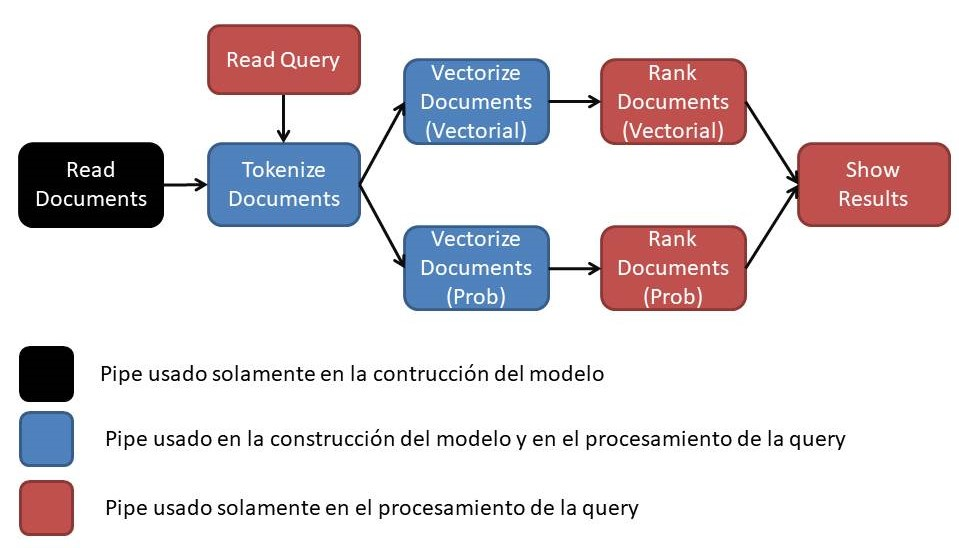
\includegraphics[width=\textwidth]{pipeline.jpg}
\caption{Ejemplo de pipelines} \label{pipeline_fig}
\end{figure}

\begin{figure}
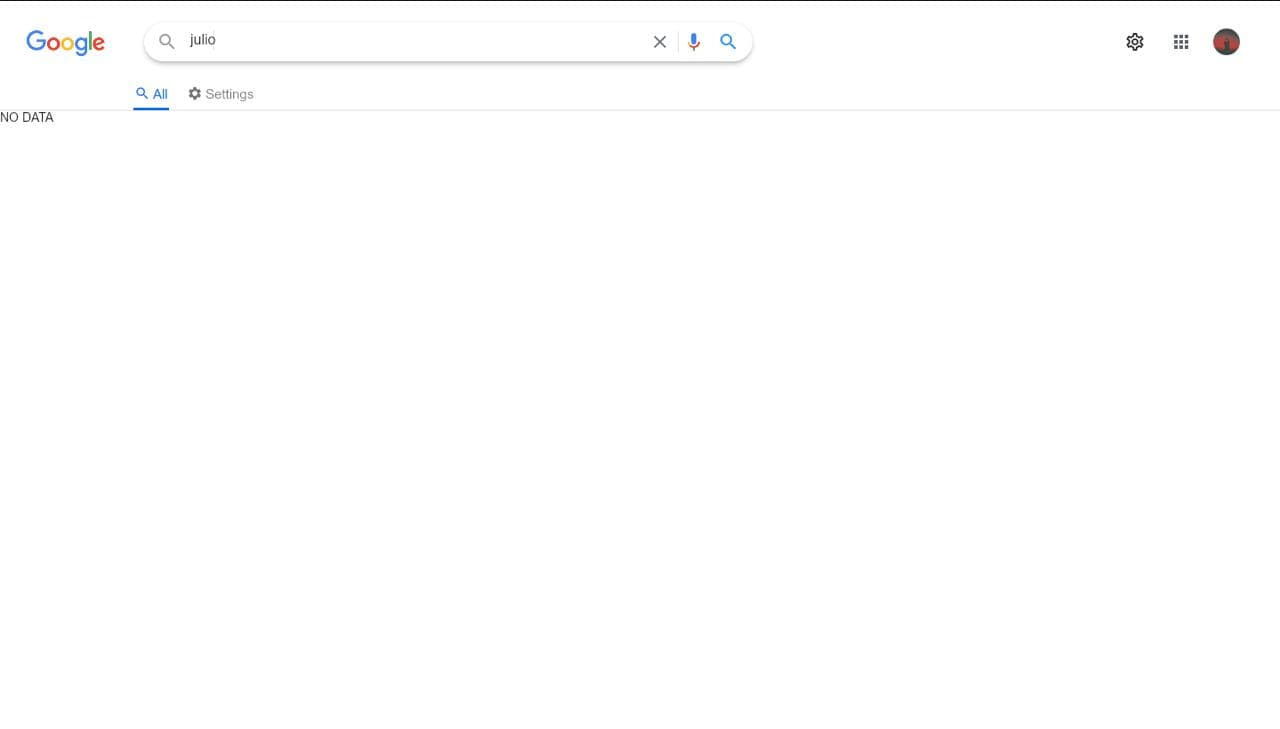
\includegraphics[width=\textwidth]{ui.jpg}
\caption{Interfaz visual Flutter} \label{ui_fig}
\end{figure}
    
\begin{figure}
    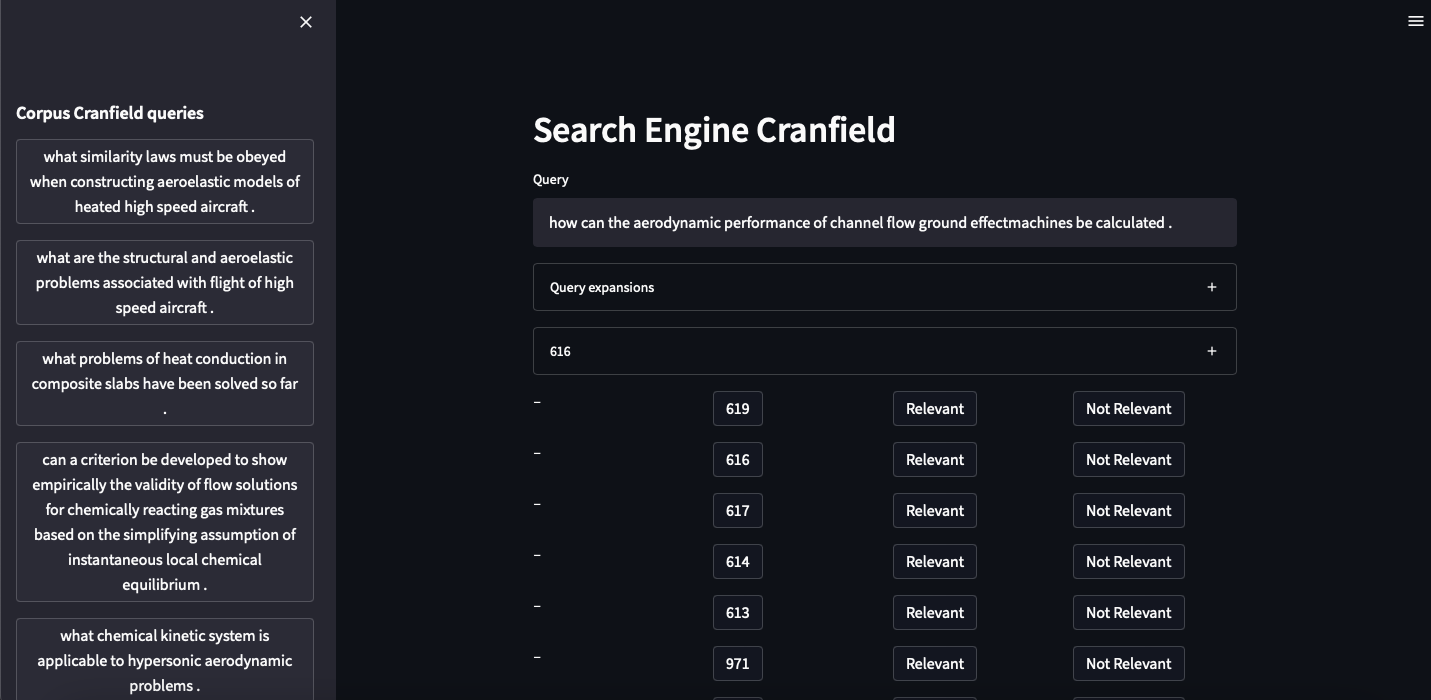
\includegraphics[width=\textwidth]{ui_streamlit.png}
    \caption{Interfaz visual streamlit} \label{ui_streamlit_fig}
\end{figure}

\newpage
        
\begin{thebibliography}{8}

\bibitem{alphaManning}
Christopher D. Manning, Prabhakar Raghavan, and Hinrich Schütze:
An Introduction to Information Retrieval. Online edition, pp. 127 Cambridge University Press,
Cambridge, England (2009) Ver página

\bibitem{lsaWiki}
Wikipedia, \url{https://en.wikipedia.org/wiki/Latent\_semantic\_analysis}. Consultado 25 de junio de 2022 Ver página

\bibitem{rankSVM}
Joachims: Optimizing Search Engines Using Clickthrough Data. In: Proceedings of the ACM Conference 
on Knowledge Discovery and Data Mining (KDD). ACM (2002) Ver página

\bibitem{svmSklearn}
Scikit Learn SVM Documentation, \url{https://scikit-learn.org/stable/modules/svm.html}. Consultado 25 de junio de 2022 Ver página 

\end{thebibliography}

\end{document}
